\section{N3: methodology-guided gap mapping}
\label{sec:n3}

N3 (\repo{gapmap/}) reads one N2 ledger and turns silences in it into inspectable candidates: a
place where the sources name a construct but do not state its content, with a hypothesis about what
a practitioner would add. \Cref{sec:architecture} describes the package's modules. This section
reports what the pipeline produced on three real N2 ledgers, and the checks that expose its central
weakness.

\evobs{} N3's registered status is \textbf{PoC pipeline complete; hidden-knowledge prediction not
demonstrated.}\footnote{\repo{research/n3/README.md}.} The registered gate that would test prediction (E-CTA,
E-OSS against held-out gold; restructured as V2 and H-OSS in \cref{sec:validation}) has not run: no gold has been acquired, and the absence check does not
beat its fair control (\cref{sec:absence-check}).

\textbf{What the lenses read.} \evobs{} Lens firing rules, the stem index, every anchor and the
judge's seed text all run on the extractor's paraphrase of a claim (its \code{assertion}), not on the
verbatim span. The knowledge types that gate DIAG, GUARD and HEDGE were also assigned by the
extractor. Spans are kept for display and for the quotes in questions.\footnote{\repo{gapmap/src/gapmap/lenses.py}
(\code{_diag_anchor}, \code{_best_sentence}); \repo{gapmap/src/gapmap/link.py};
\repo{gapmap/src/gapmap/semantic.py}.} The PoC's gap candidates are therefore built on model-written
text that is tied to, but not identical with, the source.

\subsection{The seven lenses}

Each lens names a construct drawn from the methods review (\cref{sec:foundations}) and fires when the
ledger attests that construct without stating its content. \Cref{tab:n3-lenses} summarizes them;
\cref{app:lenses} gives each firing rule and human channel.

\begin{table}[tbp]
  \centering
  \small
  \caption{The seven methodology lenses. Firing rules and elicitation channels are in
  \cref{app:lenses}.}
  \label{tab:n3-lenses}
  \begin{tabularx}{\linewidth}{@{}lXX@{}}
    \toprule
    Lens & Missing element & Predicted knowledge type \\
    \midrule
    DISC & Boundary of a judgment term & cue, perceptual or collective \\
    DIAG & A sign that tells rival causes apart & interpretation, cue \\
    SEL & Situation $\rightarrow$ option mapping & decision \\
    HEDGE & The exception condition on a hedged rule & decision \\
    GUARD & How an automated error is noticed & check, automated \\
    WHY & The rationale for a prescribed step & rationale \\
    RESULT & What a test result means and where it leads & interpretation, expectancy \\
    \bottomrule
  \end{tabularx}
\end{table}

A lens fires over criterion-labeled claims only (never over \code{synthetic_extrapolation} or
\code{unknown} claims). Each firing becomes a \emph{candidate}, not yet a gap. \evobs{} Lens firing
tracks each domain's texture, as designed: DIAG fires only on PLC, the diagnostic domain, while DISC
and HEDGE fire mainly on GDPR, the normative domain (\cref{tab:n3-firing}). This shows that the lenses
distinguish domain texture, not that they find hidden knowledge.

\begin{table}[tbp]
  \centering
  \small
  \caption{Lens firing per ledger, recomputed offline with \code{gapmap.lenses.run_all}.
  \enquote{Promotional seeds excluded} counts candidates dropped before judgment by the domain
  denylist.}
  \label{tab:n3-firing}
  \begin{tabularx}{\linewidth}{@{}lrXr@{}}
    \toprule
    Ledger & Candidates fired & By lens & Promotional seeds excluded \\
    \midrule
    PLC & 56 & WHY 24, RESULT 19, DIAG 9, SEL 2, DISC 1, GUARD 1 & 42 \\
    GDPR v1 & 51 & RESULT 21, DISC 13, WHY 8, HEDGE 5, SEL 4 & 8 \\
    GDPR v2 & 48 & DISC 14, SEL 11, RESULT 9, WHY 9, HEDGE 5 & 1 \\
    \bottomrule
  \end{tabularx}
\end{table}

\subsection{The absence check: closure}
\label{sec:absence-check}

Firing a lens only shows that a construct is named. Deciding that its content is really
\emph{unsaid} (\code{closure} in code) needs a second step. The PoC tried two versions.

\textbf{Lexical closure (first version).} A stem co-occurrence rule scored a candidate closed if
another claim shared enough stems with the missing element. \evobs{} Against a donor-claim null
(200 random-donor draws, self and same-source claims excluded from both arms), the final maps'
observed lexical-closure counts fall within or below the null's 5--95\% interval on every ledger (PLC
below it): PLC 22 against a null mean of 33.48 (26--41), GDPR v1 11 against 12.735 (8--17), GDPR v2
11 against 8.08 (5--12).\footnote{\repo{research/n3/plc/gapmap.json},
\repo{research/n3/gdpr_v1/gapmap.json}, \repo{research/n3/gdpr_v2/gapmap.json}, field
\code{checks.lexical_donor_null}; \code{CLOSURE_NULL_DRAWS} in \repo{gapmap/src/gapmap/config.py}.
Pre-final maps reported other figures; they are historical.} Lexical closure did no better than
chance.

\textbf{Semantic closure (final version).} A local judge (\code{qwen2.5:7b-instruct} over Ollama,
temperature 0, cached and replayable) reads the sentences a lexical retriever pulls from the ledger,
up to 8 verified and 4 unverified per probe, and decides whether the missing element is stated:
\code{closed}, \code{partial} or \code{open}. DIAG probes each rival cause separately, so a DIAG
record can rest on more sentences (34 and 50 in the two PLC DIAG records).

\evobs{} The map's fair control keeps the seed's own sentences in both arms and swaps only the
other-source sentences for those of the topically nearest candidate of the same lens. Lenses with
fewer than two candidates are skipped. The judge's closure rate, counting \code{partial} as closed,
is the same in both arms: \textbf{PLC 0.889, GDPR v1 0.961, GDPR v2 0.958} ($n = 54, 51, 48$).
Every tested lens in every ledger is flagged \code{closure-uninformative}
(\cref{fig:closure}).\footnote{\repo{research/n3/}\,(\code{gapmap.json} in each domain folder), field
\code{checks.mismatched_evidence_control}.}

Four qualifications keep this result in proportion.\footnote{The paired figures come from an
offline replay of the committed judge caches with the package's own functions, made for the review of
this report; they are not yet an output of \repo{gapmap/src/gapmap/checks.py}.} First, in 32 of the
153 pairs (PLC 8, GDPR v1 11, GDPR v2 13) the two arms sent the judge an identical prompt, so equality
there holds by construction. Second, the rate counts \code{partial} as closed, while triage keeps
partial candidates; counted on \code{closed} alone, own versus control is 0.30/0.33, 0.65/0.61 and
0.58/0.52, still far below the 0.20 difference the check requires. Third, the own rate is 1.0 on 11
of the 14 tested lens--ledger cells, so the test has little room to separate the arms. Fourth, an arm
with the seed's and same-source sentences removed still closes or partly closes 0.667, 0.725 and
0.708 of candidates, which fits a lenient judge as well as any other mechanism.

\evint{} The reading is narrow: the judge's verdict does not depend on which evidence it is shown,
so it is not yet an informative absence check. Every candidate should be read as \enquote{a lens
fired here}, not as \enquote{experts know something here}.

\evobs{} How this was found matters. An adversarial AI review of the pre-final maps found that the
absence check did not beat a fair control; the first built-in control had been a straw man that
\enquote{passed}. The fair control was then written into \repo{gapmap/src/gapmap/checks.py}, raised
the \code{closure-uninformative} flag on the final maps, and is re-run on every replay.

\begin{figure}[tbp]
  \centering
  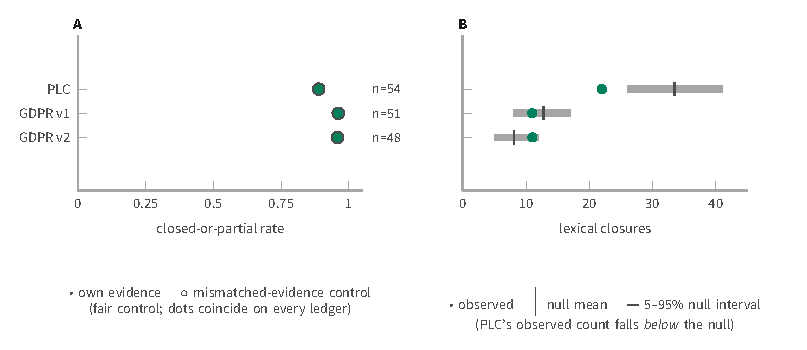
\includegraphics{figures/pdf/fig08_closure.pdf}
  \caption[The absence check versus its fair control]{Panel A: closed-or-partial rate of the
  closure judge on a candidate's own evidence and on the fair control (other-source sentences swapped
  for the topically nearest candidate's), by ledger. The rates are equal in every ledger: the judge's
  verdict does not depend on which candidate's other-source evidence it is shown. Panel B: observed
  lexical closures against the donor null (mean and 5--95\% interval of 200 draws).}
  \label{fig:closure}
\end{figure}

\subsection{Triage: retrieval gaps versus gap candidates}

A candidate that is not closed is sorted into one of two kinds (\cref{sec:evidence-model} gives the
taxonomy):

\begin{itemize}[noitemsep]
  \item \textbf{Retrieval gaps}: thin support, not a hidden-knowledge signal. \code{RG-UNK}
    (nothing found for a searched, fully examined slot), \code{RG-SINGLE} (only one independent
    source discusses the topic), \code{RG-UNVER} (closed only by an unverified or synthetic
    sentence), \code{RG-SIBLING} (the same anchor closes in an independent sibling reconstruction)
    and \code{RG-UNDECIDED} (the judge's answer could not be parsed; never defaulted to
    \code{open}). Their action is to search or verify further, not to ask a human. One GDPR v2
    \code{RG-SIBLING} record still carries a hypothesis and a question, because the sibling step
    changes the category without clearing them; this is a defect (\cref{app:defects}).
  \item \textbf{Gap candidates} (category \code{HYP}): a three-tier record of
    \code{observed_evidence} (the verbatim spans, each with its label and verdict),
    \code{inferred_gap} (the closure judgment and its reasoning, re-runnable from the cache) and
    \code{hypothesis}, a hidden-knowledge hypothesis whose label is fixed to \code{inferred}. A record
    is HYP when its state is \code{open} or \code{partial}, at least two independent sources
    discuss the topic, and no retrieval-gap rule applies first.
\end{itemize}

\subsection{Ranking, display cap and template questions}

Candidates are ranked by \textbf{breadth}, a rubric (\code{confidence_rubric} in
\repo{gapmap/src/gapmap/record.py}): score $= A + B - P - Q$, where $A$ buckets the number of
independent sources that discuss the topic, $B$ rewards step breadth, and $P$ and $Q$ penalize a
\code{partial} state and a promotional seed. It is \emph{not} expected information gain (EIG); EIG-based
selection is future work (N6). A single-source candidate becomes \code{RG-SINGLE}, never a
hypothesis.

\evobs{} After merging near-duplicate records, the map applies a display cap: at most 12 records, 3
per lens and 4 per area (\code{MAP_TOP_N}, \code{MAP_PER_LENS}, \code{MAP_PER_AREA} in
\repo{gapmap/src/gapmap/config.py}). Records beyond the cap are dropped from the output; they are
not moved to the retrieval gaps. On PLC this removes 15 of 24 merged HYP records (10 RESULT, 5 WHY);
the GDPR maps are not affected.\footnote{Offline replay of \code{rank.merge} and \code{rank.build}
from the committed judge cache.} The cap is per lens, so it also shapes the lens mix of the displayed
map. Any future area score must be computed over the uncapped set.

Each expert-facing question is \textbf{filled from a Python f-string template, not by a model
call}: a fixed interview frame (e.g., DISC: \enquote{Think of a recent case where you had to judge
whether something was \{anchor\}\ldots}) with up to two quotes from distinct independence keys. A
quote is the most relevant verbatim span sentence; when no usable sentence exists, the code falls
back to the extractor's assertion and still sets it in quotation marks (GDPR v1's only candidate is
such a case, \cref{app:records}).

\subsection{Built-in checks}

Every map carries its own checks, so a reader does not have to trust an unaudited ranking:
anti-renaming (does the ranking reproduce evidence density? Jaccard overlap with density-sorted
rankings and a Spearman correlation), the fair mismatched-evidence control and the lexical donor
null (\cref{sec:absence-check}), and cross-run stability across the two independent GDPR
reconstructions. The committed maps replay byte-identically from the committed judge caches with no
network call (\cref{app:reproduce}).

\subsection{Results per domain}

\Cref{tab:n3-results} gives the final map counts. Map lengths in the committed JSON (10, 2 and 7)
each include one \code{CONTROL} slot, which targets the area with the highest attested share that
produced no hypothesis, on top of the HYP records.

\begin{table}[tbp]
  \centering
  \small
  \caption{N3 final maps, per domain. GDPR v2 is not N3-admissible (140 of 366 evidence items kept a
  \code{pending} verdict, \cref{sec:n2}) and is shown only for the cross-run check. RG-UNK is the N3
  retrieval-gap category (it recombines unknown, thin and unverified slots at the claim level), a
  different count from N2's unknown claims in \cref{tab:n2-elive}.}
  \label{tab:n3-results}
  \begin{tabularx}{\linewidth}{@{}p{3.3cm}XXX@{}}
    \toprule
    & PLC & GDPR v1 & GDPR v2 (not admissible) \\
    \midrule
    HYP after merge (uncapped) & 24: RESULT 13, WHY 8, DIAG 2, GUARD 1 & 1: RESULT &
      6: RESULT 3, DISC 1, HEDGE 1, WHY 1 \\
    HYP shown after the display cap & 9: RESULT 3, WHY 3, DIAG 2, GUARD 1 & 1 & 6 \\
    Closure state of shown HYP & 3 open, 6 partial & 1 partial & 6 partial \\
    RG-SINGLE / RG-UNVER / RG-SIBLING / RG-UNK & 11 / 0 / n/a / 10 & 12 / 4 / 2 / 28 &
      3 / 6 / 7 / 44 \\
    \bottomrule
  \end{tabularx}
\end{table}

\evobs{} The three \code{open} records need a closer look. The two PLC DIAG records read
\code{open} although the judge marked 5 and 6 claims as partial: the DIAG rule counts a rival as
unsigned whenever its state is not \code{closed}, so a group of partially signed rivals reads
\code{open}. Only one of the 16 displayed candidates (PLC rank 7, a WHY record with three independent
sources) has no partial hit at all.\footnote{\repo{research/n3/plc/gapmap.json},
\code{map[*].inferred_gap.partial_hits}; the rule is in \code{semantic._judge_diag}.} For every
candidate, the lens fired; the absence check found the element at most partly stated.

\begin{figure}[tbp]
  \centering
  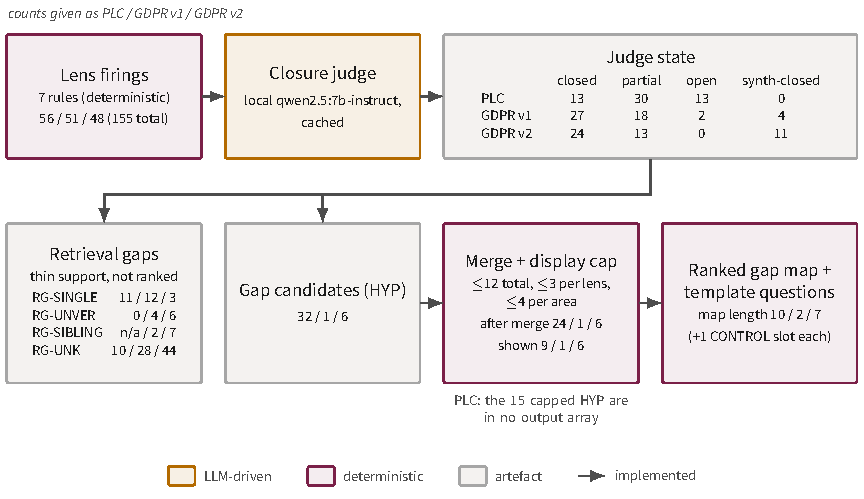
\includegraphics{figures/pdf/fig07_n3.pdf}
  \caption[From lens firing to gap candidate or nothing]{How lens firings become retrieval gaps, gap
  candidates or nothing, with counts per ledger (PLC / GDPR v1 / GDPR v2). After the closure judge
  and triage, near-duplicate HYP records are merged (PLC 24) and a display cap keeps at most 12
  records, 3 per lens and 4 per area (PLC 9 shown; GDPR unaffected). Most shown candidates are
  \code{partial}, not \code{open}.}
  \label{fig:n3}
\end{figure}

\subsection{The negative results, stated plainly}

\begin{itemize}[noitemsep]
  \item \textbf{The absence check ties its fair control on every ledger}, and lexical closure does
    no better than its donor null (\cref{sec:absence-check}).
  \item \textbf{13 of the 16 displayed gap candidates are \code{partial}}, and the two PLC DIAG
    records are \code{open} only by the DIAG rule. \evint{} The fair control counts \code{partial}
    as closed, so most surviving hypotheses sit in a state the map's own control would call
    \emph{closed}, an internal tension we state rather than hide.
  \item \textbf{Precision by adversarial judgment: 3 of 19 strict (8 of 19 lenient), on the
    pre-final maps only.} \evobs{} One adversarial AI reviewer (Opus) judged the pre-final maps'
    candidates, in-sample, with no human coder and no gold; the per-record tally is not committed.
    Wilson 95\% CIs, recomputed: 5.5--37.6\% and 23.1--63.7\%. The final maps were not re-tallied
    after two changes that altered the candidate set (the parse fix below and the fair-control
    rewrite). It is a reported sanity signal, never a measured precision of the committed maps.
  \item \textbf{PLC's ranking correlates with source density} (Spearman $\rho = 0.91$; overlap of
    the top ten with the ten highest-density candidates $J_{10} = 0.58$). \evint{} The anti-renaming
    check excludes \emph{low-density renamed} ($J_{10}$ with the lowest-density ten is 0.00), not
    \emph{high-density renamed}, so this direction is not what it was built to catch. On GDPR,
    $\rho$ is 0.09 and 0.16.\footnote{\repo{research/n3/plc/gapmap.json}, key
    \code{checks.anti_renaming}.}
  \item \textbf{Cross-run stability is low.} \evobs{} Of GDPR v1's 13 unclosed lens records (1 gap
    candidate, 12 single-source retrieval gaps), 3 have any counterpart in the independent v2
    reconstruction; of v2's 9 (6 gap candidates, 3 single-source retrieval gaps), 3 have a
    counterpart in v1. Every counterpart is partial. \evint{} The two runs are dominated by different
    independence keys, so the instability traces to retrieval, not to lens logic.
  \item \textbf{The judge-parsing defect was found by review, not by tests.} \evobs{} Unparsed
    judge answers silently defaulted to \code{open}, reported in \repo{docs/lessons.md} as 24 of 103,
    62 of 150 and 60 of 147 responses; the pre-fix caches are not committed, so these counts cannot
    be re-checked. The offline tests used a fake judge that always answered in the expected format.
    An unparsable answer now becomes \code{RG-UNDECIDED}.
\end{itemize}

\begin{findingbox}
N3's pipeline runs end to end and deterministically. Its central step does not work yet: the
absence check, which decides that a missing element is really unsaid rather than merely unquoted,
does not beat a fair, topically matched control on any tested lens in any of three ledgers. An
adversarial review found this weakness; the fair control now built into every map confirms it on
each replay. Everything downstream (hypotheses, ranking, questions) inherits it: the records are
\textbf{candidates} where a lens fired, not validated predictions of what an expert knows. The
falsifier ($\Delta$AUROC against held-out gold) has not run and should not run until closure passes a
human-labeled check. The correct reading is \emph{not demonstrated, and the current absence check is
not yet a valid instrument}, not that the human knowledge residual is unpredictable.
\end{findingbox}
